\begin{question}
\label{ex:dateex}
Write code that:

\begin{itemize}
\item print the day of the week of your birthday;
\item print the weekday of your birthdays for the next 120 years.
\end{itemize}
\end{question}

\cprotEnv\begin{solution}
\begin{ipython}
import datetime

birthday = datetime.date(1974, 10, 20)
print (birthday.weekday()) # remember it starts form 0
\end{ipython}
\begin{ioutput}
6
\end{ioutput}
\begin{ipython}
from dateutil.relativedelta import relativedelta

for i in range(120):
    print ((birthday + relativedelta(years=i)).weekday())
\end{ipython}
\begin{ioutput}
6
0
2
3
4
5
0
1
2
3
4
...
\end{ioutput}
\end{solution}

\begin{question}
Write code to determine whether a given year is a leap year and test it with 1800, 1987 and 2020.

\noindent\textbf{Hint:} a leap year is divisible by 4, by 100 and by 400.
\end{question}

\cprotEnv\begin{solution}
\begin{ipython}
years = [1800, 1987, 2020]

for y in years:
    if y % 400 == 0:
        print ("{} is a leap year".format(y))
	elif y % 100 == 0:
        print ("{} is a leap year".format(y)) 
    elif y % 4 == 0:
        print ("{} is a leap year".format(y))
    else:
        print ("{} is NOT a leap year".format(y))
\end{ipython}
\begin{ioutput}
1800 is NOT a leap year
1987 is NOT a leap year
2020 is a leap year        
\end{ioutput}  
\end{solution}

\begin{question}
Write code to print next five days starting from today.
\end{question}

\cprotEnv\begin{solution}
\begin{ipython}
d = datetime.date.today()
for i in range(1, 6):
     print (d + relativedelta(days=i))
\end{ipython}
\begin{ioutput}
2020-08-04
2020-08-05
2020-08-06
2020-08-07
2020-08-08
\end{ioutput}
\end{solution}

\begin{question}
Build again dates as in Exercise~\ref{ex:dateex} (i.e. the weekday of your birthdays for the next 120 years) and count how many of your birthdays is a Monday, Tuesday, \ldots{} , Sunday until 120 years of age. Print out the result using a dictionary. (expected output something like: \texttt{\{6:\ 10,\ 0:\ 10,\ 2:\ 9,\ 3:\ 10,\ 4:\ 10,\ 5:\ 10,\ 1:\ 9\}})
\end{question}

\cprotEnv\begin{solution}
\begin{ipython}
import datetime
from dateutil.relativedelta import relativedelta

birthday = datetime.date(1974, 10, 20)
d = {}
for i in range(120):
    wd = (birthday + relativedelta(years=i)).weekday() 
    if wd in d.keys():
        d[wd] += 1
    else:
        d[wd] = 1
        
print (d)
\end{ipython}
\begin{ioutput}
{6: 17, 0: 18, 2: 17, 3: 17, 4: 17, 5: 17, 1: 17}
\end{ioutput}
\end{solution}

\begin{question}
Write an algorithm which takes in input a start date and a number of months, and returns a list of dates with \textbf{annual} frequency from the start date to the ending of the period after the specified number of months.

For example
\begin{itemize}
\item 2019-11-10 start date 12 months \(\rightarrow\) 2019-11-10, 2020-11-10
\item 2019-11-10 start date 24 months \(\rightarrow\) 2019-11-10, 2020-11-10, 2021-11-10
\end{itemize}

Note that if the number of months is not a multiple of 12, the last period should simply be shorter than 12 months. For example:

\begin{itemize}
\item 2019-11-10 start date 9 months \(\rightarrow\) 2019-11-10, 2020-08-10
\item 2019-11-10 start date 15 months \(\rightarrow\) 2019-11-10, 2020-11-10, 2021-02-10
\end{itemize}

%\begin{figure}
%  %\centering
%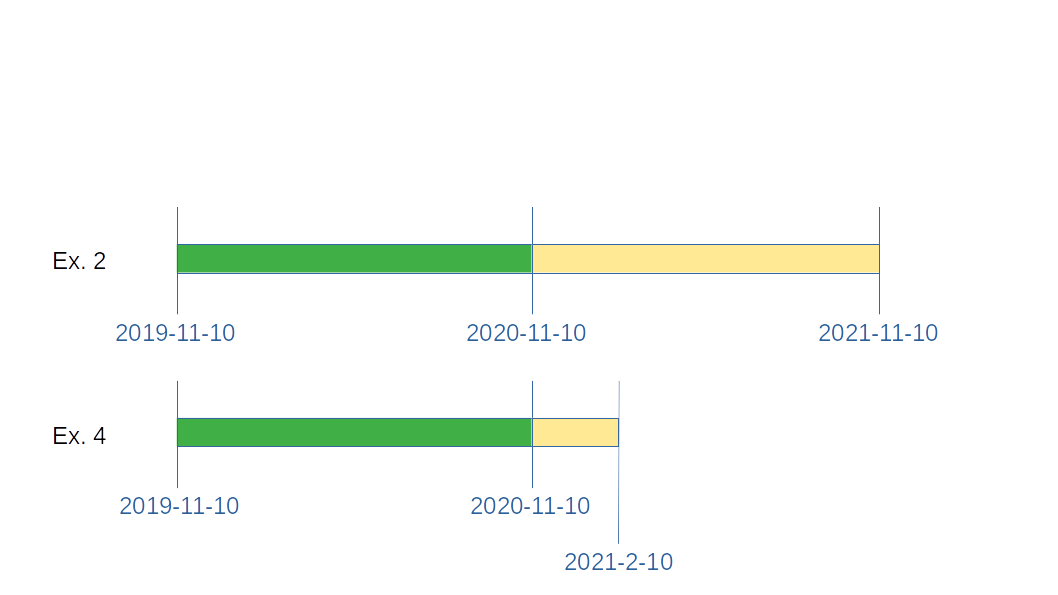
\includegraphics[width=0.8\linewidth]{time_flow.png}
%\end{figure}

%Here's some skeleton code to help you get started:
%
%\begin{Shaded}
%\begin{Highlighting}[]
%\ImportTok{from}\NormalTok{ dateutil }\ImportTok{import}\NormalTok{ relativedelta}
%
%\KeywordTok{def}\NormalTok{ generate_swap_dates(start_date, n_months):}
%\NormalTok{    dates }\OperatorTok{=}\NormalTok{ []}
%    \CommentTok{# your code here which adds all the relevant dates to the dates list}
%    \ControlFlowTok{return}\NormalTok{ dates}
%\end{Highlighting}
%\end{Shaded}
%
%\begin{Shaded}
%\begin{Highlighting}[]
%\CommentTok{# some tests to check if the function is working correctly}
%\ImportTok{from}\NormalTok{ datetime }\ImportTok{import}\NormalTok{ date}
%
%\ControlFlowTok{assert}\NormalTok{ generate_swap_dates(date(}\DecValTok{2019}\NormalTok{, }\DecValTok{11}\NormalTok{, }\DecValTok{10}\NormalTok{), }\DecValTok{12}\NormalTok{) }\OperatorTok{==}\NormalTok{ [date(}\DecValTok{2019}\NormalTok{, }\DecValTok{11}\NormalTok{, }\DecValTok{10}\NormalTok{), }
%\NormalTok{                                                       date(}\DecValTok{2020}\NormalTok{, }\DecValTok{11}\NormalTok{, }\DecValTok{10}\NormalTok{)]}
%\ControlFlowTok{assert}\NormalTok{ generate_swap_dates(date(}\DecValTok{2019}\NormalTok{, }\DecValTok{11}\NormalTok{, }\DecValTok{10}\NormalTok{), }\DecValTok{24}\NormalTok{) }\OperatorTok{==}\NormalTok{ [date(}\DecValTok{2019}\NormalTok{, }\DecValTok{11}\NormalTok{, }\DecValTok{10}\NormalTok{), }
%\NormalTok{                                                       date(}\DecValTok{2020}\NormalTok{, }\DecValTok{11}\NormalTok{, }\DecValTok{10}\NormalTok{), }
%\NormalTok{                                                       date(}\DecValTok{2021}\NormalTok{, }\DecValTok{11}\NormalTok{, }\DecValTok{10}\NormalTok{)]}
%
%\ControlFlowTok{assert}\NormalTok{ generate_swap_dates(date(}\DecValTok{2019}\NormalTok{, }\DecValTok{11}\NormalTok{, }\DecValTok{10}\NormalTok{), }\DecValTok{9}\NormalTok{) }\OperatorTok{==}\NormalTok{ [date(}\DecValTok{2019}\NormalTok{, }\DecValTok{11}\NormalTok{, }\DecValTok{10}\NormalTok{), }
%\NormalTok{                                                      date(}\DecValTok{2020}\NormalTok{, }\DecValTok{8}\NormalTok{, }\DecValTok{10}\NormalTok{)]}
%\ControlFlowTok{assert}\NormalTok{ generate_swap_dates(date(}\DecValTok{2019}\NormalTok{, }\DecValTok{11}\NormalTok{, }\DecValTok{10}\NormalTok{), }\DecValTok{15}\NormalTok{) }\OperatorTok{==}\NormalTok{ [date(}\DecValTok{2019}\NormalTok{, }\DecValTok{11}\NormalTok{, }\DecValTok{10}\NormalTok{), }
%\NormalTok{                                                       date(}\DecValTok{2020}\NormalTok{, }\DecValTok{11}\NormalTok{, }\DecValTok{10}\NormalTok{), }
%\NormalTok{                                                       date(}\DecValTok{2021}\NormalTok{, }\DecValTok{2}\NormalTok{, }\DecValTok{10}\NormalTok{)]}
%\end{Highlighting}
%\end{Shaded}
\end{question}

\cprotEnv\begin{solution}
\begin{ipython}
from datetime import date
from dateutil.relativedelta import relativedelta

start_dates} = date(2019, 11, 10)
n_months = 15
dates = []
for i in range(0, n_months, 12):
    dates.append(start_date + relativedelta(months=i))
dates.append(start_date + relativedelta(months=n_months))

print(dates)
\end{ipython}
\begin{ioutput}
[date(2019, 11, 10), date(2020, 11, 10), date(2021, 2, 10)]
\end{ioutput}
\end{solution}

%\begin{solution}
%\begin{Verbatim}[commandchars=\\\{\}]
%\PY{k+kn}{from} \PY{n+nn}{finmarkets} \PY{k}{import} \PY{n}{generate\PYZus{}swap\PYZus{}dates}
%\PY{k+kn}{from} \PY{n+nn}{datetime} \PY{k}{import} \PY{n}{date}
%\PY{k+kn}{from} \PY{n+nn}{dateutil}\PY{n+nn}{.}\PY{n+nn}{relativedelta} \PY{k}{import} \PY{n}{relativedelta}
%
%\PY{k}{def} \PY{n+nf}{generate\PYZus{}swap\PYZus{}dates}\PY{p}{(}\PY{n}{start\PYZus{}date}\PY{p}{,} \PY{n}{n\PYZus{}months}\PY{p}{)}\PY{p}{:}
%    \PY{n}{dates} \PY{o}{=} \PY{p}{[}\PY{p}{]}
%    \PY{k}{for} \PY{n}{i} \PY{o+ow}{in} \PY{n+nb}{range}\PY{p}{(}\PY{l+m+mi}{0}\PY{p}{,} \PY{n}{n\PYZus{}months}\PY{p}{,} \PY{l+m+mi}{12}\PY{p}{)}\PY{p}{:}
%        \PY{n}{dates}\PY{o}{.}\PY{n}{append}\PY{p}{(}\PY{n}{start\PYZus{}date} \PY{o}{+} \PY{n}{relativedelta}\PY{p}{(}\PY{n}{months}\PY{o}{=}\PY{n}{i}\PY{p}{)}\PY{p}{)}
%    \PY{n}{dates}\PY{o}{.}\PY{n}{append}\PY{p}{(}\PY{n}{start\PYZus{}date} \PY{o}{+} \PY{n}{relativedelta}\PY{p}{(}\PY{n}{months}\PY{o}{=}\PY{n}{n\PYZus{}months}\PY{p}{)}\PY{p}{)}
%    
%    \PY{k}{return} \PY{n}{dates}
%
%
%\PY{k}{assert} \PY{n}{generate\PYZus{}swap\PYZus{}dates}\PY{p}{(}\PY{n}{date}\PY{p}{(}\PY{l+m+mi}{2019}\PY{p}{,} \PY{l+m+mi}{11}\PY{p}{,} \PY{l+m+mi}{10}\PY{p}{)}\PY{p}{,} \PY{l+m+mi}{12}\PY{p}{)} \PY{o}{==} \PY{p}{[}\PY{n}{date}\PY{p}{(}\PY{l+m+mi}{2019}\PY{p}{,} \PY{l+m+mi}{11}\PY{p}{,} \PY{l+m+mi}{10}\PY{p}{)}\PY{p}{,} 
%                                                       \PY{n}{date}\PY{p}{(}\PY{l+m+mi}{2020}\PY{p}{,} \PY{l+m+mi}{11}\PY{p}{,} \PY{l+m+mi}{10}\PY{p}{)}\PY{p}{]}
%\PY{k}{assert} \PY{n}{generate\PYZus{}swap\PYZus{}dates}\PY{p}{(}\PY{n}{date}\PY{p}{(}\PY{l+m+mi}{2019}\PY{p}{,} \PY{l+m+mi}{11}\PY{p}{,} \PY{l+m+mi}{10}\PY{p}{)}\PY{p}{,} \PY{l+m+mi}{24}\PY{p}{)} \PY{o}{==} \PY{p}{[}\PY{n}{date}\PY{p}{(}\PY{l+m+mi}{2019}\PY{p}{,} \PY{l+m+mi}{11}\PY{p}{,} \PY{l+m+mi}{10}\PY{p}{)}\PY{p}{,} 
%                                                       \PY{n}{date}\PY{p}{(}\PY{l+m+mi}{2020}\PY{p}{,} \PY{l+m+mi}{11}\PY{p}{,} \PY{l+m+mi}{10}\PY{p}{)}\PY{p}{,} 
%                                                       \PY{n}{date}\PY{p}{(}\PY{l+m+mi}{2021}\PY{p}{,} \PY{l+m+mi}{11}\PY{p}{,} \PY{l+m+mi}{10}\PY{p}{)}\PY{p}{]}
%
%\PY{k}{assert} \PY{n}{generate\PYZus{}swap\PYZus{}dates}\PY{p}{(}\PY{n}{date}\PY{p}{(}\PY{l+m+mi}{2019}\PY{p}{,} \PY{l+m+mi}{11}\PY{p}{,} \PY{l+m+mi}{10}\PY{p}{)}\PY{p}{,} \PY{l+m+mi}{9}\PY{p}{)} \PY{o}{==} \PY{p}{[}\PY{n}{date}\PY{p}{(}\PY{l+m+mi}{2019}\PY{p}{,} \PY{l+m+mi}{11}\PY{p}{,} \PY{l+m+mi}{10}\PY{p}{)}\PY{p}{,} 
%                                                      \PY{n}{date}\PY{p}{(}\PY{l+m+mi}{2020}\PY{p}{,} \PY{l+m+mi}{8}\PY{p}{,} \PY{l+m+mi}{10}\PY{p}{)}\PY{p}{]}
%\PY{k}{assert} \PY{n}{generate\PYZus{}swap\PYZus{}dates}\PY{p}{(}\PY{n}{date}\PY{p}{(}\PY{l+m+mi}{2019}\PY{p}{,} \PY{l+m+mi}{11}\PY{p}{,} \PY{l+m+mi}{10}\PY{p}{)}\PY{p}{,} \PY{l+m+mi}{15}\PY{p}{)} \PY{o}{==} \PY{p}{[}\PY{n}{date}\PY{p}{(}\PY{l+m+mi}{2019}\PY{p}{,} \PY{l+m+mi}{11}\PY{p}{,} \PY{l+m+mi}{10}\PY{p}{)}\PY{p}{,} 
%                                                               \PY{n}{date}\PY{p}{(}\PY{l+m+mi}{2020}\PY{p}{,} \PY{l+m+mi}{11}\PY{p}{,} \PY{l+m+mi}{10}\PY{p}{)}\PY{p}{,} 
%                                                               \PY{n}{date}\PY{p}{(}\PY{l+m+mi}{2021}\PY{p}{,} \PY{l+m+mi}{2}\PY{p}{,} \PY{l+m+mi}{10}\PY{p}{)}\PY{p}{]}
%\end{Verbatim}
%\end{solution}
